\documentclass[11pt]{article}
\usepackage[letterpaper,margin=0.80in]{geometry}
\usepackage{amsmath,amssymb,mathtools,bm,amsthm}
\usepackage{microtype,setspace,caption,titlesec,enumitem,booktabs,array}
\usepackage{graphicx,tikz-cd,hyperref,xcolor}
\usepackage{balance}
\setstretch{1.05}
\setlength{\parskip}{0.27em}
\setlength{\parindent}{1.1em}
\setlength{\columnsep}{0.28in}
\setlength{\emergencystretch}{2em}
\raggedbottom
\captionsetup{font=small,labelfont=bf}
\titleformat{\section}{\large\bfseries\raggedright\hyphenpenalty=10000}{\thesection}{0.55em}{}
\titleformat{\subsection}{\normalsize\bfseries\raggedright\hyphenpenalty=10000}{\thesubsection}{0.5em}{}
\titlespacing*{\section}{0pt}{1em}{0.4em}
\titlespacing*{\subsection}{0pt}{0.75em}{0.3em}
\newtheorem{proposition}{Proposition}
\newcommand{\R}{\mathbb R}
\newcommand{\Z}{\mathbb Z}
\newcommand{\SO}{\mathrm{SO}}
\newcommand{\U}{\mathrm U}
\newcommand{\n}{\bm n}
\newcommand{\uu}{\bm u}
\newcommand{\ww}{\bm w}
\newcommand{\et}{\bm e_\theta}
\newcommand{\el}{\bm e_\lambda}
\newcommand{\Ag}{A^{\rm g}}
\newcommand{\sinc}{\operatorname{sinc}}
\hypersetup{hidelinks,
pdftitle={Spatial Dimension, Internal Phase, and Kinematics of Helical Line Families},
pdfauthor={Xiaodan Wu},
pdfsubject={Geometric tools for effective spatial dimension and phase-bearing rollout},
pdfkeywords={spatial dimension, helix, internal phase, circle bundle, kinematics, frame transport, The Emergent Frame},
pdfinfo={ORCID={0009-0005-5892-0293},Version={2.1},DOI={10.5281/zenodo.22945612}}}
\title{\bfseries Spatial Dimension, Internal Phase, and Kinematics of Helical Line Families}
\author{\normalsize Xiaodan Wu\textsuperscript{*}\\[-0.02em]\small Independent Researcher}
\date{\footnotesize September 2026\quad Preprint, Version 2.1}
\begin{document}
\twocolumn[
\begin{@twocolumnfalse}
\maketitle
\vspace{-0.9em}
\begin{center}\textbf{Abstract}\end{center}
\noindent
A helical curve is intrinsically one-dimensional, while a family of helices can carry both three-dimensional position labels and an internal phase. We formulate this distinction using an origin-referenced parameter base and a directional frame bundle. On a selected regular local position chart, the state space is a circle bundle over a three-dimensional effective position image; this dimension is conditional on the chosen position map, not a physical dimension derived from helicity. Independent phase is retained throughout. A connection defines pathwise phase comparison and loop compatibility, and a moving-frame calculation gives velocity and acceleration for arbitrary position--phase paths. A constant-radius realization maps this four-dimensional state space to three-dimensional ambient positions with rank three, so its pullback metric is degenerate and its position cannot determine a complete state. After selecting a common initial phase in a specified frame, an explicit injective domain and a closed-form inverse yield ordinary three-dimensional helical coordinates. Their Euclidean pullback metric is flat, while finite-resolution averages can retain tangent and arc-length effects even when position displacements are small. We relate axis-transverse and curve-normal frames explicitly, and distinguish local manifold dimension from the conditional volume-growth dimension of published The Emergent Frame (TEF) rollout constructions. The result is a geometric and kinematic toolkit for spatial dimension and relative state, with physical dynamics and quantum-state interpretation left to separate applications.
\par\vspace{0.55em}
\noindent\textbf{Keywords:} spatial dimension; helix; internal phase; circle bundle; relative spatial state; moving frame; coordinate transformation; rollout geometry.
\vspace{1em}
\end{@twocolumnfalse}
]
\begingroup
\renewcommand{\thefootnote}{\fnsymbol{footnote}}
\footnotetext[1]{\raggedright
\href{mailto:xiaodan@theemergentframe.org}{xiaodan@theemergentframe.org}\\
\href{https://theemergentframe.org}{theemergentframe.org}; ORCID: \href{https://orcid.org/0009-0005-5892-0293}{0009-0005-5892-0293}.\\
DOI: \href{https://doi.org/10.5281/zenodo.22945612}{10.5281/zenodo.22945612}.}
\endgroup

\section{Question and mathematical lineage}

If a straight coordinate line is replaced by a helix and a common origin labels a family of directions, what is the resulting spatial dimension? The answer requires distinguishing a curve, a position map, and the states carried over its image. The present paper develops that distinction into coordinate and transport tools for The Emergent Frame (TEF), while stating the mathematical assumptions independently of a physical mechanism for spatial rollout.

The historical starting point is the separation of intrinsic geometry from extrinsic bending in the work of Gauss and Riemann \cite{Gauss,Riemann}. A regular curve has one local parameter even when its curvature and torsion are nonzero \cite{doCarmo}. Moving frames, including Bishop frames, separate the geometry of a curve from a choice of transverse axes \cite{Bishop,Hornung}. These ideas motivate retaining an orientation variable without counting it automatically as another spatial direction.

Cosserat continua provide a classical precedent for translational position accompanied by local rotational data \cite{Cosserat}. Cartan geometry supplies a language of coframes, connections, curvature, and torsion; the spiral-staircase example realizes helical transport in three dimensions \cite{LazarHehl}. Neither precedent makes a helical drawing evidence of nonzero spatial curvature or torsion. Those quantities require a specified metric or connection.

Fiber bundles formalize the local separation of position and internal orientation \cite{Steenrod}. In the present construction the fiber is a circle. Its status differs from a compact coordinate explicitly included in a higher-dimensional spacetime metric, as in Kaluza's construction \cite{Kaluza}. The role assigned to a coordinate depends on the projection and observables, not just parameter counting. Discrete exterior calculus and analytic probes of dimension supply complementary tools for relational realizations \cite{Desbrun,Carlip}.

We first keep the full phase-bearing state space, then select a phase section to obtain an explicit coordinate example. This ordering distinguishes general kinematics from a restricted family of coordinate lines. It also separates coordinate changes, which preserve the encoded motion, from averages, which may discard information. The ingredients are standard mathematical tools; the contribution is their explicit organization, domain analysis, and application to this family.

\section{Curve, position, and state dimensions}

\subsection{One curve and a three-parameter base}

A nondegenerate circular helix may be written
\begin{equation}
 \begin{gathered}
 h(\varphi)=(R\cos\varphi,R\sin\varphi,a\varphi),\\
 R>0,\qquad a\ne0.
 \end{gathered}
\end{equation}
Its line element is $d\ell^2=(R^2+a^2)d\varphi^2$. After arc-length reparametrization its intrinsic metric is simply $d\ell^2$; its intrinsic dimension is one. The radius and axial advance per radian specify its shape, not extra curve coordinates.

Let $I$ be an open interval, $O$ a reference origin, and $\n\in S^2$ a mean direction. Define
\begin{equation}
 B=I\times S^2,\qquad F:B\longrightarrow\R^3.
 \label{eq:F}
\end{equation}
A representative effective position assignment is
\begin{equation}
 F(s,\n)=O+z(s)\n.
 \label{eq:radialF}
\end{equation}
The origin fixes a coordinate reference; it imposes no requirement that a microscopic helix pass through $O$.

\begin{proposition}[Local effective position]
If $\operatorname{rank}dF=3$ at a point of $B$, then $F$ restricts to a diffeomorphism from a neighborhood $U$ onto an open image $M_{\rm eff}\subset\R^3$. For \eqref{eq:radialF}, $z\ne0$ and $z'\ne0$ suffice.
\end{proposition}
\begin{proof}
The base has dimension $1+2=3$. Its longitudinal derivative is $z'\n$, while its angular derivatives span the transverse plane when $z\ne0$. The inverse function theorem gives the stated local image.
\end{proof}
Thus three-dimensionality is a conditional result for the chosen effective position construction. It is not inferred from one helix. In the explicit calculations below, $I=(0,\infty)$ and $z(r)=r$.

\subsection{Retaining the circle of orientations}

Choose an oriented transverse unit vector $\uu\perp\n$. The pair $(\n,\uu)$, together with $\ww=\n\times\uu$, specifies an oriented frame. The full state space and its base projection are
\begin{equation}
 \begin{aligned}
 P&=I\times\SO(3),\\
 p:P&\longrightarrow B,\quad(s,\n,\uu)\mapsto(s,\n).
 \end{aligned}
 \label{eq:P}
\end{equation}
The circle action rotates $\uu$ about $\n$, leaving $p$ fixed. Over a regular chart of $F$, set $P_U=p^{-1}(U)$ and $\pi_U=F\circ p$. Then
\begin{equation}
 \begin{gathered}
 S^1\hookrightarrow P_U\xrightarrow{\pi_U}M_{\rm eff},\\
 \dim P_U=4,\qquad\dim M_{\rm eff}=3.
 \end{gathered}
 \label{eq:bundle}
\end{equation}
Since $dp$ has rank three and $F|_U$ is a diffeomorphism,
\begin{equation}
 \operatorname{rank}d\pi_U=3,\qquad
 \dim\ker d\pi_U=1.
 \label{eq:rankpi}
\end{equation}
The global bundle initially asserted is $\SO(2)\hookrightarrow\SO(3)\to S^2$ over directions, with the interval factor included. Its interpretation over effective positions is established here only on the selected regular chart.

\begin{equation}
 \begin{tikzcd}[column sep=1.8em,row sep=1.2em]
 P_U\arrow[r,"p"]\arrow[dr,"\pi_U"']&U\arrow[d,"F|_U"]\\
 &M_{\rm eff}
 \end{tikzcd}
 \label{eq:diagram}
\end{equation}
Effective position is therefore the quotient $P_U/\SO(2)$ under this assignment. Quotienting by position does not assert that orientation states are indistinguishable by all measurements. Their physical identity requires observables. Nor is the assignment yet identified with a period average or measurement coarse graining.

\begin{table*}[t]
\centering\small
\begin{tabular}{@{}>{\raggedright\arraybackslash}p{0.24\textwidth}>{\raggedright\arraybackslash}p{0.14\textwidth}>{\raggedright\arraybackslash}p{0.56\textwidth}@{}}
\toprule
Object & Dimension & Role\\
\midrule
Single helical member & 1 & One intrinsic curve parameter.\\
Direction sphere $S^2$ & 2 & Two angles label a mean direction.\\
Regular effective image $M_{\rm eff}$ & 3 & Rank-three position map on a chosen chart.\\
Circle fiber $S^1$ & 1 & Orientation at a fixed assigned position.\\
State space $P_U$ & 4 & Position labels and independently variable phase.\\
Selected phase section & 3 & A restricted family; its realization is a coordinate chart only where injective and regular.\\
Volume-growth exponent $d_f$ & Model dependent & An analytic property of a metric-measure realization, distinct from local manifold dimension.\\
\bottomrule
\end{tabular}
\caption{Dimension bookkeeping. Four state parameters do not supply a fourth effective spatial translation or a time coordinate.}
\label{tab:dim}
\end{table*}

\subsection{Effective position and ambient realization}

On a direction patch choose $(\bm e_1,\bm e_2)$ with $\bm e_1\times\bm e_2=\n$. Write
\begin{equation}
 \uu=\cos\chi\,\bm e_1+\sin\chi\,\bm e_2.
 \label{eq:u}
\end{equation}
For fixed $R>0$, the following is a second map:
\begin{equation}
 H:P\longrightarrow\R^3,\qquad
 H(r,\n,\uu)=O+r\n+R\uu.
 \label{eq:H}
\end{equation}
It is globally defined on $(0,\infty)\times\SO(3)$ even though a single phase coordinate is not. In particular,
\begin{equation}
 |H-F|=R,\qquad |H-O|^2=r^2+R^2.
 \label{eq:norm}
\end{equation}
Changing phase at fixed $(r,\n)$ changes $H$ but leaves $\pi_U$ fixed. The two position maps must therefore not be interchanged.

A chosen section with $\chi=r/a+\psi_*$ traces circular helices at fixed $\n$, where $a>0$ fixes handedness and $\psi_*$ is an initial phase in this frame. More general sections need not trace circular helices. Likewise, replacing $R,r$ by functions $\rho(s),z(s)$ produces general axis-winding curves; the formulas below explicitly specialize to constant $R$ and $z(r)=r$.

\section{Phase comparison and transport}

\subsection{Reference changes and the geometric connection}

A passive transverse-frame rotation by $\alpha$ sends
\begin{equation}
 \chi'=\chi-\alpha.
\end{equation}
The same $\uu$ then has a different angular coordinate. A local connection $A$ transforms as $A'=A+d\alpha$, making
\begin{equation}
 \omega_A=d\chi+A
 \label{eq:omega}
\end{equation}
frame invariant. This connection supplies a horizontal comparison of states, independent of which phase section is selected.

The embedded direction-frame construction supplies a useful particular choice,
\begin{equation}
 \Ag=\bm e_2\cdot d\bm e_1,
 \qquad \omega_{\rm g}=d\chi+\Ag.
 \label{eq:Ag}
\end{equation}
It is the pullback of the round direction-sphere frame connection. Another connection on the same bundle has the form $A=\Ag+k$, with $k$ a base one-form, subject to the same patching. Covariance does not determine $k$ or its dynamics. The explicit Euclidean realization kinematics uses $\Ag$, not an arbitrary substituted $A$.

Let
\begin{equation}
 \eta=\uu\cdot d\n,\qquad\zeta=\ww\cdot d\n.
 \label{eq:coframe}
\end{equation}
Differentiating the orthonormal frame yields
\begin{equation}
 \begin{aligned}
 d\n&=\uu\eta+\ww\zeta,\\
 d\uu&=-\n\eta+\ww\omega_{\rm g},\\
 d\ww&=-\n\zeta-\uu\omega_{\rm g}.
 \end{aligned}
 \label{eq:frameeq}
\end{equation}
These equations retain the independent phase through $d\chi$.

\subsection{Pathwise comparison and loop compatibility}

For a path $\gamma_{ij}$ in one trivialization, define
\begin{equation}
 \Delta^{\rm cov}_{\gamma_{ij}}\chi
 =\chi_j-\chi_i+\int_{\gamma_{ij}}A
 \pmod{2\pi}.
 \label{eq:comparison}
\end{equation}
This is invariant under the stated reference change. For a path crossing charts, parallel transport composes local expressions and transition rotations. A connection specifies comparison along a path, not a path-independent phase difference. In a common chart, the loop factor is $\exp(i\oint A)$; for a contractible loop bounding a surface in that chart, Stokes' theorem relates it to $dA$. Globally, patch transitions must be included.

\begin{proposition}[Compatibility of discrete phase locking]
On a connected comparison graph, choose link angles $\mathfrak a_{ij}$ in the convention of \eqref{eq:comparison}, with $\mathfrak a_{ji}=-\mathfrak a_{ij}$ modulo $2\pi$. Vertex phases satisfying
\begin{equation}
 \chi_j-\chi_i+\mathfrak a_{ij}=0\pmod{2\pi}
 \label{eq:locking}
\end{equation}
on every oriented edge exist if and only if every graph cycle has trivial holonomy. They are unique up to a common phase.
\end{proposition}
\begin{proof}
Summing \eqref{eq:locking} around a cycle cancels vertex phases, proving necessity. Conversely choose a root phase and transport it along graph paths. Trivial cycle holonomy makes the answer path independent and satisfies every edge equation. Connectedness gives uniqueness up to the root value.
\end{proof}
This is the graph version of the phase-locking boundary identified in the source-local rollout geometry study \cite{WuGeometry}. Numerical equality of phases in a chart is not the same condition as \eqref{eq:locking}. A common initial phase is a chosen section; it need not be horizontal for $A$.

Globally on the full direction sphere, no smooth nonvanishing transverse vector field exists. The state bundle describes available orientations, not a globally selected coherent field. Restricted domains, multiple representations of compatible local data, or defects must be specified. Multiple charts alone do not remove the obstruction to a global section.

\section{Kinematics with an independent phase}

\subsection{Velocity and acceleration of a state path}

For an externally parametrized state path $\gamma_P(t)\in P$, set
\begin{equation}
 \eta_t=\uu\cdot\dot\n,\quad
 \zeta_t=\ww\cdot\dot\n,\quad
 \nu=\dot\chi+\Ag(\dot b),
 \label{eq:rates}
\end{equation}
where $b(t)=(r(t),\n(t))$ is its base path. These three angular rates are invariant under changes of transverse reference. When using another comparison connection $A=\Ag+k$, its covariant phase rate is $\nu_A=\nu+k(\dot b)$; the rate entering the embedded frame equations remains $\nu$.

The effective and realization velocities are
\begin{equation}
 \dot{\bar{\bm X}}=\dot r\n+r\dot\n,
 \label{eq:effectivevelocity}
\end{equation}
and
\begin{equation}
 \begin{aligned}
 \dot{\bm X}&=v_n\n+v_u\uu+v_w\ww,\\
 v_n&=\dot r-R\eta_t,\\
 v_u&=r\eta_t,\\
 v_w&=r\zeta_t+R\nu,
 \qquad \bm X=H(\gamma_P(t)).
 \end{aligned}
 \label{eq:velocityfull}
\end{equation}
Using \eqref{eq:frameeq} gives the full acceleration
\begin{equation}
 \begin{aligned}
 \ddot{\bm X}={}&(\dot v_n-\eta_t v_u-\zeta_t v_w)\n\\
 &+(\dot v_u+\eta_t v_n-\nu v_w)\uu\\
 &+(\dot v_w+\zeta_t v_n+\nu v_u)\ww.
 \end{aligned}
 \label{eq:accelfull}
\end{equation}
Thus the phase rate and its derivative are retained rather than absorbed into a fixed coordinate choice. Equations \eqref{eq:velocityfull}--\eqref{eq:accelfull} follow directly by differentiating \eqref{eq:H}; they impose no equation of motion.

At fixed mean direction, $\eta_t=\zeta_t=0$. In a direction-only reference frame, $\nu=\dot\chi$, so
\begin{equation}
 \begin{aligned}
 \dot{\bm X}&=\dot r\n+R\dot\chi\ww,\\
 \ddot{\bm X}&=\ddot r\n-R\dot\chi^2\uu
                   +R\ddot\chi\ww.
 \end{aligned}
 \label{eq:fixedaxis}
\end{equation}
Writing $\chi=r/a+\psi(t)$ displays both the native rollout contribution $\dot r/a$ and the independent phase contribution $\dot\psi$. Only when $\psi$ is constant is the fixed-initial-phase motion recovered.

\subsection{Why a full-state inverse is unavailable}

\begin{proposition}[Rank of the full realization]
For $r>0$ and $R>0$, the full map $H$ has rank three. Its differential has a one-dimensional kernel that differs from the circle-fiber kernel of $d\pi_U$.
\end{proposition}
\begin{proof}
In the coframe $(dr,\eta,\zeta,\omega_{\rm g})$,
\begin{equation}
 dH=\n(dr-R\eta)+\uu(r\eta)
                         +\ww(r\zeta+R\omega_{\rm g}).
 \label{eq:dHfull}
\end{equation}
Its matrix has rows $(1,-R,0,0)$, $(0,r,0,0)$, and $(0,0,r,R)$, so its rank is three. The kernel satisfies $dr=\eta=0$ and $r\zeta+R\omega_{\rm g}=0$. In contrast, the circle-fiber generator has $dr=\eta=\zeta=0$, $\omega_{\rm g}=1$, and is mapped by $dH$ to $R\ww\ne0$.
\end{proof}

Accordingly, $H$ is not locally one-to-one on complete states. The Euclidean pullback on $P$ is
\begin{equation}
 G_H=(dr-R\eta)^2+r^2\eta^2
                    +(r\zeta+R\omega_{\rm g})^2.
 \label{eq:degenerate}
\end{equation}
It has rank three and is not a positive-definite four-dimensional state metric. The effective Euclidean pullback $dr^2+r^2(\eta^2+\zeta^2)$ is also degenerate on $P$, but along the vertical phase direction. A nondegenerate state metric or an independent phase energy would require additional data.

This distinction is operationally relevant: a complete state path determines an effective position path and an ambient realization path, while the latter alone generally does not reconstruct the complete state. Neither is yet a transport law for a TEF excitation.

\section{Selected phase sections and coordinates}
\label{sec:coordinates}

\subsection{Common initial phase as a restricted family}

Choose the meridional frame on $0<\theta<\pi$:
\begin{equation}
 \begin{aligned}
 \n&=(\sin\theta\cos\lambda,\sin\theta\sin\lambda,\cos\theta),\\
 \et&=\partial_\theta\n,
 \qquad\el=(-\sin\lambda,\cos\lambda,0).
 \end{aligned}
\end{equation}
It has $\Ag=\cos\theta\,d\lambda$, and hence
\begin{equation}
 d\Ag=-\sin\theta\,d\theta\wedge d\lambda.
 \label{eq:angularcurvature}
\end{equation}
For a loop bounding an oriented surface inside this frame chart, $\oint\Ag$ is minus its signed solid angle. This is curvature of directional phase comparison; it does not imply curvature of the ambient Euclidean metric.

Let $a>0$ and select the section $\sigma_{\psi_*}$ defined by
\begin{equation}
 \chi=r/a+\psi_*,\qquad\psi_*\text{ constant}.
 \label{eq:section}
\end{equation}
This constraint is a choice of states in a specified frame, not a removal of the phase freedom from $P$. Under a passive frame change the same section generally has nonconstant initial-phase coordinates. The parameter $a$ selects the winding of this section; the full available-state map \eqref{eq:H} did not require it.

Set $h_*=H\circ\sigma_{\psi_*}$, $\bm y=h_*-O$, $C=\cos\chi$, $S=\sin\chi$, and
\begin{equation}
 D=r\sin\theta+RC\cos\theta.
\end{equation}
The Cartesian realization is
\begin{equation}
 \begin{aligned}
 y_x+i y_y&=e^{i\lambda}(D+iRS),\\
 y_z&=r\cos\theta-RC\sin\theta.
 \end{aligned}
 \label{eq:cartesian}
\end{equation}

\begin{proposition}[Regular and injective section]
The section realization $h_*$ has determinant
\begin{equation}
 \det\frac{\partial\bm y}{\partial(r,\theta,\lambda)}=rD.
 \label{eq:det}
\end{equation}
For any $0<\theta_0<\pi/2$, it is injective modulo azimuthal periodicity on
\begin{equation}
 \begin{gathered}
 r>R\cot\theta_0,\qquad
 \theta_0<\theta<\pi-\theta_0,\\
 \lambda\in S^1.
 \end{gathered}
 \label{eq:belt}
\end{equation}
Cutting the azimuth gives ordinary coordinate charts. The domain is sufficient, not maximal.
\end{proposition}
\begin{proof}
Differentiating \eqref{eq:cartesian}, or using the Jacobian in Appendix~\ref{app:cartesian}, gives \eqref{eq:det}. On \eqref{eq:belt}, $D\ge r\sin\theta-R|\cos\theta|>0$. The norm identity \eqref{eq:norm} fixes the unique positive $r$ from the image. With $r$ fixed, $C,S$ are fixed and $\partial_\theta y_z=-D<0$, so $\theta$ is unique. Finally $D+iRS\ne0$ determines $\lambda$ modulo $2\pi$. Regularity and uniqueness give a smooth inverse on the image.
\end{proof}

For a point in that image the inverse is explicit:
\begin{equation}
 \begin{aligned}
 r&=\sqrt{|\bm y|^2-R^2},\qquad\chi=r/a+\psi_*,\\
 d&=\sqrt{r^2+R^2\cos^2\chi},\\
 \delta&=\operatorname{atan2}(R\cos\chi,r),\\
 \theta&=\arccos(y_z/d)-\delta,\\
 \lambda&=\operatorname{atan2}(y_y,y_x)\\
 &\quad-\operatorname{atan2}(R\sin\chi,D)\pmod{2\pi}.
 \end{aligned}
 \label{eq:inverse}
\end{equation}
The positive-$D$ branch satisfies $0<\theta+\delta<\pi$. For arbitrary input, check $|\bm y|>R$, the arccosine range, the strict inequalities \eqref{eq:belt}, and the azimuth cut. The image does not cover the origin or the radius-$R$ ball; $O$ remains a reference zero.

Common origin and initial phase alone do not ensure injectivity. For $R=a=r=1$ and $\psi_*=-1$, the distinct points $(1,2\pi/3,0)$ and $(1,5\pi/6,\pi)$ share an image although both have nonzero Jacobian. Between those branches, $D=0$ at $\theta=3\pi/4$ and an azimuthal circle collapses. This is a failure of the selected section map; the full $H$ still has rank three there.

\begin{figure*}[t]
\centering
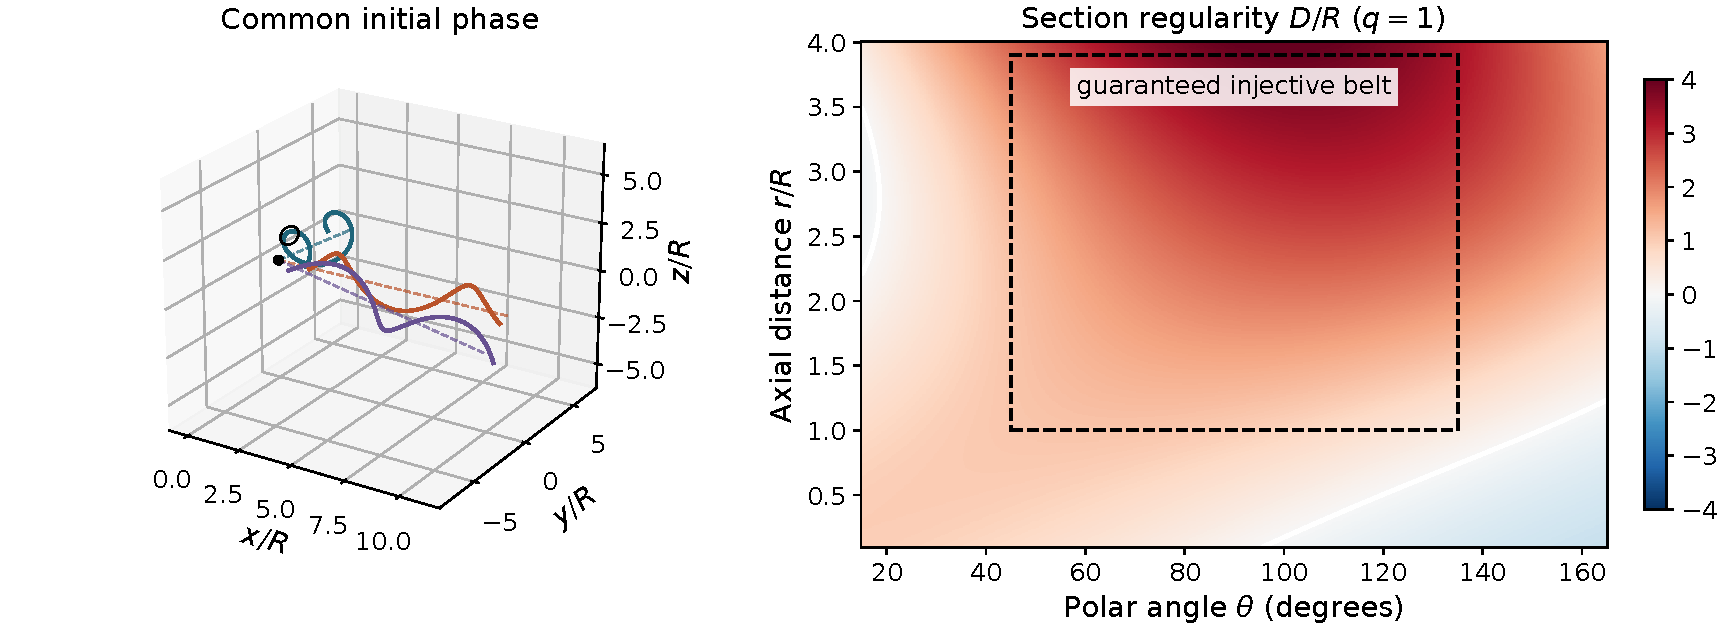
\includegraphics[width=0.96\textwidth]{../figures/coordinates_v2.pdf}
\caption{A common-initial-phase coordinate example. Left: three helices with distinct mean directions, with dashed axial labels. Right: signed regularity factor $D/R$ for $a/R=1$ and $\psi_*=0$. White curves mark $D=0$; the dashed rectangle lies in the sufficient injective belt $\theta_0=\pi/4$, $r/R>1$. Regularity of this selected three-dimensional section is different from the rank-three full-state map.}
\label{fig:coords}
\end{figure*}

\subsection{Metric and the same motion in two charts}

On the section, $\omega_{\rm g}=dr/a+\Ag$. Thus
\begin{equation}
 \begin{aligned}
 g_*={}&(dr-R\eta)^2+r^2\eta^2\\
      &+\bigl((R/a)dr+R\Ag+r\zeta\bigr)^2.
 \end{aligned}
 \label{eq:metricsection}
\end{equation}
This is positive definite where $rD\ne0$ and has zero Riemann curvature there: it is the Euclidean pullback by a local diffeomorphism. Its volume element is $|rD|dr\,d\theta\,d\lambda$. This exact finite-radius flatness concerns the selected Euclidean realization, not a derived physical metric of all TEF rollout structures.

Let $\xi=(r,\theta,\lambda)$, $J_i=\partial_i h_*$, and $K_{ij}=\partial_i\partial_jh_*$. Then
\begin{equation}
 \begin{aligned}
 \dot{\bm X}&=J_i\dot\xi^i,\\
 \ddot{\bm X}&=J_i\ddot\xi^i+K_{ij}\dot\xi^i\dot\xi^j,\\
 \ddot\xi&=J^{-1}\bigl(\ddot{\bm X}-K_{ij}\dot\xi^i\dot\xi^j\bigr).
 \end{aligned}
 \label{eq:chartkin}
\end{equation}
The associated connection is $\Gamma^k{}_{ij}=(J^{-1})^k{}_\alpha K^\alpha{}_{ij}$. A Cartesian uniform straight trajectory has $\ddot{\bm X}=0$ and obeys the resulting coordinate geodesic equation while it remains in the chart. Holding direction angles fixed and increasing $r$ uniformly instead traces a physical helix. Those are different trajectories. In this comparison the Cartesian point is $h_*(\xi)$; $F(\xi)$ is its axial label, not the same ambient point.

\section{Axis-transverse and curve-normal frames}

The transverse pair above is orthogonal to the mean axis $\n$. The source-local rollout geometry construction instead attaches a normal pair to the actual curve tangent \cite{WuGeometry}. An explicit bridge is available for a native circular member with fixed $\n,\psi_*$.

Let $q=a/R>0$. Its Frenet tangent, normal, and binormal are
\begin{equation}
 \begin{aligned}
 \bm T&=\frac{q\n+\ww}{\sqrt{1+q^2}},\\
 \bm N&=-\uu,\qquad
 \bm B=\frac{\n-q\ww}{\sqrt{1+q^2}}.
 \end{aligned}
 \label{eq:framebridge}
\end{equation}
They form a positively oriented orthonormal frame, but $\bm T\ne\n$ at finite $q$. With arc length $\ell$,
\begin{equation}
 \begin{aligned}
 \frac{d\ell}{dr}&=\sqrt{1+q^{-2}},\\
 \kappa_h&=\frac{1}{R(1+q^2)},\qquad
 \tau_h=\frac{q}{R(1+q^2)},\\
 \bm B\cdot d\bm N&=\tau_h\,d\ell
       =\frac{dr}{R\sqrt{1+q^2}}.
 \end{aligned}
 \label{eq:bridgeconnection}
\end{equation}
These relations agree with the circular-helix invariants used in the gravity-calibrated helix, neutrino correspondence, and rollout geometry studies \cite{WuHelix,WuNeutrino,WuGeometry}. The mean-axis frame may be constant along this line, while the Frenet normal frame rotates. Their connection coefficients must not be identified solely because both comparison groups are $\SO(2)$.

Equation \eqref{eq:framebridge} relates the triads of this prescribed circular member. It does not identify the two circle-fiber actions: rotation around $\n$ generally changes $\bm T$, whereas rotation of a normal frame about a fixed $\bm T$ does not. Nor is the formula the Frenet frame of an arbitrary path with variable $\n$ or independent $\psi(t)$. Such a path is handled by \eqref{eq:velocityfull}--\eqref{eq:accelfull}; its tangent, when defined, follows from its actual velocity. Additional frame-transport choices are required for a general microscopic correspondence.

\section{Finite radius and finite resolution}

\subsection{Position closeness and tangent persistence}

At fixed direction on the native phase section,
\begin{equation}
 \left|\frac{dh_*}{dr}-\frac{dF}{dr}\right|=q^{-1},
 \qquad (g_*)_{rr}=1+q^{-2}.
 \label{eq:nonuniform}
\end{equation}
The position displacement is only $R$, but the tangent difference does not decrease with $r/R$ at fixed $q$. As $R\to0$ with $a=qR$, positions converge uniformly to the axial curve on fixed intervals, while their first derivatives do not. For monotone $r$,
\begin{equation}
 L_{\rm helix}=\sqrt{1+q^{-2}}\,|r_2-r_1|.
\end{equation}
This factor persists at fixed shape. Taking $q\to\infty$ is a different limit that suppresses the tangent correction.

For uniform fixed-direction motion $r=r_0+vt$, $v>0$, on the native section, $\Omega=v/a$ and
\begin{equation}
 \dot{\bm X}=v\n+R\Omega\ww,\qquad
 \ddot{\bm X}=-R\Omega^2\uu.
\end{equation}
If its helical speed is a prescribed $c>0$, then
\begin{equation}
 \begin{aligned}
 v&=\frac{cq}{\sqrt{1+q^2}},\qquad P_{\rm turn}=2\pi qR,\\
 T&=\frac{2\pi R\sqrt{1+q^2}}{c}.
 \end{aligned}
 \label{eq:scales}
\end{equation}
These are ordinary helix relations also used in the gravity-calibrated helical spacetime ansatz \cite{WuHelix}. The mathematical construction leaves $R,q,c$ free. The ansatz's gravity calibration $R_G=\ell_{\rm P}/2$ and its shape-closure condition can be inserted for an application; neither is needed for the rank or kinematic results. Along a general phase path, the total angular rate is not fixed by $v/a$, so \eqref{eq:scales} is not a universal period law.

\subsection{A bound valid with independent phase}

\begin{proposition}[Endpoint and averaged-velocity error]
For any state path $\gamma_P(t)$ and $\Delta=t_2-t_1>0$, let $\bar{\bm X}(t)=(F\circ p)(\gamma_P(t))$ denote the effective path. Then
\begin{equation}
 \begin{aligned}
 &|\bm X(t_2)-\bm X(t_1)\\
 &\qquad-\bar{\bm X}(t_2)+\bar{\bm X}(t_1)|\le2R.
 \end{aligned}
 \label{eq:endpoint}
\end{equation}
For continuously differentiable paths, their time-averaged velocities differ by at most $2R/\Delta$.
\end{proposition}
\begin{proof}
Subtract the endpoint values of $\bm X-\bar{\bm X}=R\uu$ and use $|\uu|=1$. The fundamental theorem of calculus gives the velocity statement. No phase locking, fixed direction, or constant speed is required.
\end{proof}
These are absolute bounds. Relative errors require a nonzero reference scale. They give no bound on arbitrary instantaneous phase rates or accelerations.

\subsection{A specified average for the native member}

For uniform fixed-direction motion only, define the centered box average over a window wholly inside its time domain:
\begin{equation}
 \langle f\rangle_\Delta(t)=\frac1\Delta
 \int_{t-\Delta/2}^{t+\Delta/2}f(s)\,ds.
\end{equation}
Direct integration gives
\begin{equation}
 \begin{aligned}
 \langle\bm X\rangle_\Delta&=\bar{\bm X}
          +R\sinc(\Omega\Delta/2)\uu,\\
 \langle\dot{\bm X}\rangle_\Delta&=v\n
          +R\Omega\sinc(\Omega\Delta/2)\ww,\\
 \langle\ddot{\bm X}\rangle_\Delta&=-R\Omega^2
                     \sinc(\Omega\Delta/2)\uu,
 \end{aligned}
 \label{eq:averages}
\end{equation}
where $\sinc x=\sin x/x$, continuously extended at zero. Integer multiples of $T=2\pi/\Omega$ eliminate all three transverse means in this example. For arbitrary windows,
\begin{equation}
 \begin{aligned}
 |\langle\dot{\bm X}\rangle_\Delta-v\n|&\le2R/\Delta,\\
 |\langle\ddot{\bm X}\rangle_\Delta|&\le2R\Omega/\Delta.
 \end{aligned}
 \label{eq:averagebounds}
\end{equation}
At fixed $q,c,\Delta$ the second bound is independent of $R$, and the exact acceleration need not converge as $R\to0$. Convergence of averaged velocity therefore does not establish convergence of acceleration with the same box window. Scalar speed remains $c$ even when the mean velocity is exactly $v\n$.

The relevant ratios are $R/r$ for angular displacement from the axial label, $R/L$ for position resolution at reference length $L$, $P_{\rm turn}/L$ for axial turn resolution, and $T/\Delta$ for temporal averaging. None alone is a universal classical--microscopic boundary. For a varying envelope, a hierarchy $T\ll\Delta\ll\tau_{\rm slow}$ motivates further analysis but does not constitute a proved effective dynamics here. In particular, a position average need not erase loop holonomy or relative-phase data retained as separate observables.

\begin{figure*}[t]
\centering
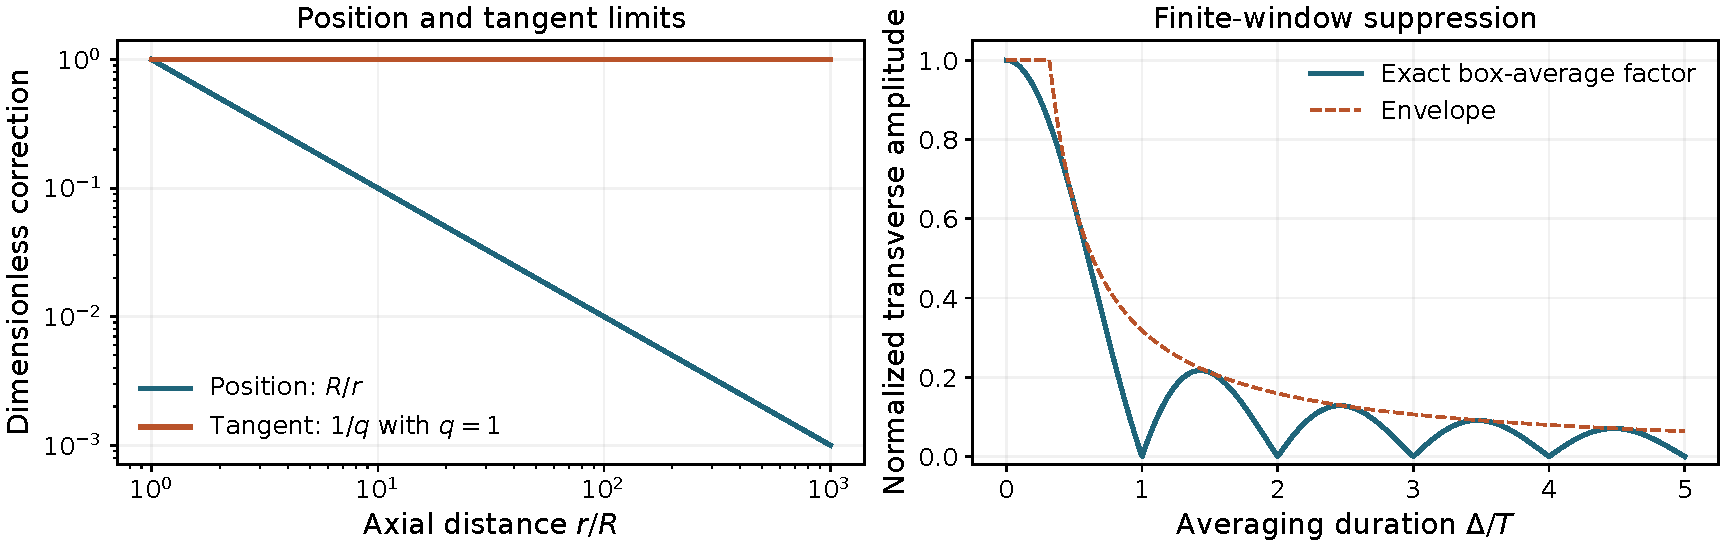
\includegraphics[width=0.96\textwidth]{../figures/scales_v2.pdf}
\caption{Distinct scale limits for the native fixed-initial-phase member. Left: the relative position displacement $R/r$ decreases while the tangent correction remains $1/q$ (shown for $q=1$). Right: the box-average factor $|\sinc(\pi\Delta/T)|$ and its envelope. Phase, velocity, and acceleration cannot be discarded solely on the basis of small position displacement.}
\label{fig:scales}
\end{figure*}

\section{Relation to published TEF structures}

\subsection{What is inherited and what is supplied here}

Earlier TEF studies supply distinct ingredients. The relative-framing model of the matter--space interface formulates transverse framing as an $S^1$ variable and distinguishes reference-dependent phase lifts from relative classes \cite{WuMatter}. The minimal rollout framework separates rollout reference phase from excitation-dependent quantum phase, and requires transport for phase comparison \cite{WuFramework}. The source-local rollout geometry study retains transverse phase and gluing holonomy after intrinsic untwisting, and defines covariant multi-line coherence \cite{WuGeometry}. The connection-dynamics model of an effective electromagnetic sector adopts compact links and loop curvature as geometric input to a separately assumed effective Hamiltonian \cite{WuEM}.

This paper supplies a continuous position--phase state space, its effective projection, arbitrary-phase kinematics, and a selected-section coordinate calculation. It does not identify the round direction-sphere connection $\Ag$ with the independent dynamical connection in the effective electromagnetic model \cite{WuEM}. Their relationship, including frame choice and any additional one-form $k$, must be specified by an application.

To compare link conventions with the rollout geometry study \cite{WuGeometry}, write its transport from the $j$ fiber to the $i$ fiber as $U_{ij}=e^{-ia_{ij}}$, with $\chi_i\mapsto\chi_i-\alpha_i$. Then $a_{ij}'=a_{ij}+\alpha_i-\alpha_j$. Setting $\mathfrak a_{ij}=-a_{ij}$ makes its invariant $\chi_j-\chi_i-a_{ij}$ identical to \eqref{eq:comparison}. This sign is a transport-direction convention, not a new physical difference.

\subsection{Local dimension and growth dimension}

The source-local rollout geometry study \cite{WuGeometry} proves, under its transported weighted-complex assumptions,
\begin{equation}
 \mathcal K\cong\Z_{\rm cell}\times\mathcal K_\perp.
\end{equation}
With transverse quadratic growth and the stated uniform metric-measure conditions, this gives cubic large-scale volume growth, $d_f=3$. Additional analytic assumptions are used there for normal diffusion and the bulk $1/r$ Green scale \cite{WuGeometry}. The transverse organization is an input to that construction, not a consequence of a single normal plane.

Here $\dim M_{\rm eff}=3$ instead follows locally from the rank of $F$. The two dimension statements are compatible targets but not identical theorems. A correspondence would require sampling or reconstruction maps and metric-measure control between the continuous position charts and the relational complex. The present Euclidean example does not establish that correspondence or a global physical metric. Adding an internal phase preserves the chosen position projection; it does not by itself settle the spectral or growth dimensions of a dynamical state-space model.

\subsection{Scope of internal phase}

The compact phase here describes transverse orientation and its covariant comparison. It does not by itself select $SU(2)$ orientation completion, a Hilbert-space state, or quantum probabilities. The fine-structure correspondence study treats the spinorial lift as an additional assumption \cite{WuAlpha}; the strong-interaction confinement study adopts a formal effective Hilbert space for a separate closure problem \cite{WuStrong}. The model of an electron-like charged-textured excitation introduces collective excitation and frame-texture fields on a prescribed background, rather than identifying the primitive phase with a complete wavefunction \cite{WuElectron}.

The present tools are inputs that such applications can use. A phase-dependent action, excitation transport law, invariant observables, and the operational status of the position projection remain separate choices. Source-local language does not require the reference origin of this calculation to be a microscopic emitting point through which every helix passes.

\section{Conclusion and remaining geometric tasks}

A helix remains a one-dimensional curve. A regular chosen effective position map gives a three-dimensional local base, and its transverse orientation gives a circle of states over each base point. The resulting local state dimension is four, while the effective position dimension is three. Position and phase comparisons are relative to charts, local frames, and specified transport paths.

Keeping phase independent yields explicit full-state velocity and acceleration formulas. Its ambient realization has rank three and cannot encode a complete state uniquely; the corresponding full-state pullback is degenerate. Selecting a common initial phase gives a three-dimensional section for which we prove an injective domain and obtain an explicit inverse. Its Euclidean realization is flat at finite radius. Small position offsets nevertheless do not guarantee small tangent corrections or interchangeable averaging of all kinematic quantities.

The next geometric tasks are controlled variable-radius and variable-pitch extensions, compatible changes of reference origin, and a continuous--discrete correspondence with rollout complexes. General phase evolution requires a stated dynamical law. These tasks preserve the distinction between spatial dimension, internal state, and physical interpretation without expanding the present construction into a theory of quantum excitations or Lorentzian spacetime.

\appendix
\section{Cartesian derivatives on the selected section}
\label{app:cartesian}

Let $b=R/a$ and use $C,S,D$ from Sec.~\ref{sec:coordinates}. Resolved in the moving ambient basis $(\n,\et,\el)$, the Jacobian is
\begin{equation}
 [J_r\ J_\theta\ J_\lambda]=
 \begin{pmatrix}
 1&-RC&-RS\sin\theta\\
 -bS&r&-RS\cos\theta\\
 bC&0&D
 \end{pmatrix}.
 \label{eq:J}
\end{equation}
The six Cartesian Hessian vectors, subsequently resolved in that basis, are
\begin{equation}
 \begin{aligned}
 K_{rr}&=-R\uu/a^2,\\
 K_{r\theta}&=\et+bS\n,\\
 K_{r\lambda}&=-bC\sin\theta\n-bC\cos\theta\et\\
 &\quad+(\sin\theta-bS\cos\theta)\el,\\
 K_{\theta\theta}&=-r\n-RC\et,\\
 K_{\theta\lambda}&=(r\cos\theta-RC\sin\theta)\el,\\
 K_{\lambda\lambda}&=-D\sin\theta\n-D\cos\theta\et-RS\el.
 \end{aligned}
 \label{eq:K}
\end{equation}
They already include derivatives of the moving basis. For a Cartesian velocity $\bm V$, let $V_z$ be its fixed $z$ component and $V_\lambda=\bm V\cdot\el$. On the positive-$D$ chart,
\begin{equation}
 \begin{aligned}
 \dot r&=\frac{\bm y\cdot\bm V}{r},\\
 \dot\theta&=\frac{(\cos\theta+bS\sin\theta)\dot r-V_z}{D},\\
 \dot\lambda&=\frac{V_\lambda-bC\dot r}{D}.
 \end{aligned}
\end{equation}
For a prescribed independent phase $\psi(t)$, the four-parameter map additionally has
\begin{equation}
 \begin{aligned}
 H_\psi&=R\ww,\qquad H_{\psi\psi}=-R\uu,\\
 H_{r\psi}&=-R\uu/a,\qquad H_{\theta\psi}=RS\n,\\
 H_{\lambda\psi}&=-RC\sin\theta\n-RC\cos\theta\et\\
 &\quad-RS\cos\theta\el.
 \end{aligned}
 \label{eq:phasederivatives}
\end{equation}
Together with the fixed-$\psi$ derivatives above, these give the ordinary four-variable chain rule equivalent to \eqref{eq:velocityfull}--\eqref{eq:accelfull}. They do not define a four-by-four inverse from Cartesian position.

\section{Verification and reproducibility}

The accompanying versioned script independently differentiates the Cartesian map and checks the fixed-section Jacobian, Hessians, determinant, and metric. It checks the independent-phase derivatives and moving-frame kinematics, the distinction between the two differential kernels, the circular-member frame bridge, and reference invariance. Numerical tests include section forward/inverse round trips, Cartesian straight trajectories, freely varying phase trajectories, graph locking and frustrated loops, and quadrature of the box averages. These checks support the implementation; the propositions have analytic proofs in the text. The script, generated figures, and check results accompany the manuscript. No external physical data are needed to reproduce them.

\clearpage
\balance
\begingroup
\footnotesize\raggedright
\setlength{\parskip}{0pt}
\begin{thebibliography}{99}
\bibitem{Gauss} C. F. Gauss, ``Disquisitiones generales circa superficies curvas,'' \emph{Commentationes Societatis Regiae Scientiarum Gottingensis Recentiores} \textbf{6}, 99--146 (1828); presented 1827.
\bibitem{Riemann} B. Riemann, ``Ueber die Hypothesen, welche der Geometrie zu Grunde liegen,'' habilitation lecture (1854), published in \emph{Abhandlungen der K\"oniglichen Gesellschaft der Wissenschaften zu G\"ottingen} \textbf{13} (1868).
\bibitem{doCarmo} M. P. do Carmo, \emph{Differential Geometry of Curves and Surfaces}, Prentice--Hall (1976).
\bibitem{Bishop} R. L. Bishop, ``There is More than One Way to Frame a Curve,'' \emph{American Mathematical Monthly} \textbf{82}, 246--251 (1975), \href{https://doi.org/10.1080/00029890.1975.11993807}{doi:10.1080/00029890.1975.11993807}.
\bibitem{Hornung} P. Hornung, ``Framed Curves, Ribbons, and Parallel Transport on the Sphere,'' \emph{Journal of Nonlinear Science} \textbf{33}, 72 (2023), \href{https://doi.org/10.1007/s00332-023-09930-0}{doi:10.1007/s00332-023-09930-0}.
\bibitem{Cosserat} E. Cosserat and F. Cosserat, \emph{Th\'eorie des corps d\'eformables}, A. Hermann et Fils (1909).
\bibitem{LazarHehl} M. Lazar and F. W. Hehl, ``Cartan's spiral staircase in physics and, in particular, in the gauge theory of dislocations,'' \emph{Foundations of Physics} \textbf{40}, 1298--1325 (2010), \href{https://doi.org/10.1007/s10701-010-9440-4}{doi:10.1007/s10701-010-9440-4}.
\bibitem{Steenrod} N. Steenrod, \emph{The Topology of Fibre Bundles}, Princeton University Press (1951).
\bibitem{Kaluza} T. Kaluza, ``Zum Unit\"atsproblem der Physik,'' \emph{Sitzungsberichte der Preussischen Akademie der Wissenschaften}, 966--972 (1921); English translation, arXiv:1803.08616.
\bibitem{Desbrun} M. Desbrun, A. N. Hirani, M. Leok, and J. E. Marsden, \emph{Discrete Exterior Calculus}, arXiv:math/0508341 (2005).
\bibitem{Carlip} S. Carlip, ``Dimension and dimensional reduction in quantum gravity,'' \emph{Universe} \textbf{5}, 83 (2019), \href{https://doi.org/10.3390/universe5030083}{doi:10.3390/universe5030083}.
\bibitem{WuHelix} X. Wu, \emph{A Helical Spacetime Ansatz Linking the Planck Scale and Electroweak Mixing}, v5.1, Zenodo (2026), \href{https://doi.org/10.5281/zenodo.22101000}{doi:10.5281/zenodo.22101000}.
\bibitem{WuAlpha} X. Wu, \emph{From a Gravity-Calibrated Helix to a Conditional Fine-Structure Correspondence}, v4.7, Zenodo (2026), \href{https://doi.org/10.5281/zenodo.22117153}{doi:10.5281/zenodo.22117153}.
\bibitem{WuNeutrino} X. Wu, \emph{From a Gravity-Calibrated Helix to Neutrino Oscillation Correspondences}, v4.2, Zenodo (2026), \href{https://doi.org/10.5281/zenodo.22150998}{doi:10.5281/zenodo.22150998}.
\bibitem{WuMatter} X. Wu, \emph{Closed Matter and Open Space: A Relative-Framing Ansatz for Incomplete Quark Sectors and the Matter--Space Interface}, v4.6, Zenodo (2026), \href{https://doi.org/10.5281/zenodo.22256714}{doi:10.5281/zenodo.22256714}.
\bibitem{WuStrong} X. Wu, \emph{From a Gravity-Calibrated Helix to a Strong-Interaction Confinement Correspondence}, v4.1, Zenodo (2026), \href{https://doi.org/10.5281/zenodo.22412464}{doi:10.5281/zenodo.22412464}.
\bibitem{WuFramework} X. Wu, \emph{The Emergent Frame: A Minimal Framework for Spacetime Rollout, Interaction, and Excitation}, v2.5, Zenodo (2026), \href{https://doi.org/10.5281/zenodo.22723329}{doi:10.5281/zenodo.22723329}.
\bibitem{WuGeometry} X. Wu, \emph{Spacetime as Source-Local Rollout and the Conditional Emergence of Three-Dimensional Effective Geometry in The Emergent Frame}, v3.12, Zenodo (2026), \href{https://doi.org/10.5281/zenodo.22776137}{doi:10.5281/zenodo.22776137}.
\bibitem{WuEM} X. Wu, \emph{Rollout Connection Dynamics and a Maxwell--Lorentz-Compatible Low-Energy Electromagnetic Sector in The Emergent Frame}, v3.3, Zenodo (2026), \href{https://doi.org/10.5281/zenodo.22849547}{doi:10.5281/zenodo.22849547}.
\bibitem{WuElectron} X. Wu, \emph{An Electron-Like Charged-Textured Excitation with Spinorial Configuration Topology in The Emergent Frame}, v4.0, Zenodo (2026), \href{https://doi.org/10.5281/zenodo.22923781}{doi:10.5281/zenodo.22923781}.
\end{thebibliography}
\endgroup
\end{document}
